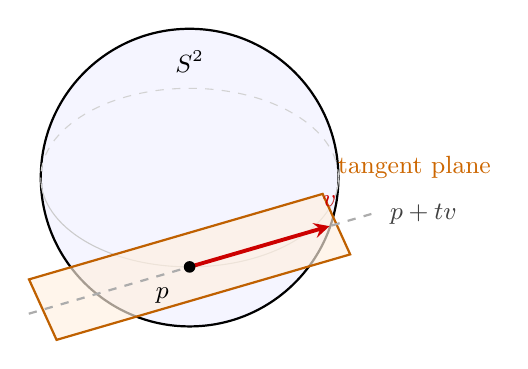
\begin{tikzpicture}[>=stealth, scale=1.05,
    x={(1.8cm,0cm)}, y={(0cm,1.44cm)}, z={(0cm,-1.08cm)}]
  % Use the same sphere projection as the curve-velocity figure.
  \draw[thick, fill=blue!4] (0,0) circle[radius=1.8cm];
  \draw[gray!35, dashed] (1.8cm,0cm) arc (0:180:1.8cm and 1.08cm);
  \draw[gray!40] (-1.8cm,0cm) arc (180:360:1.8cm and 1.08cm);
  \node[font=\small] at (0cm,1.4cm) {$S^2$};

  % The affine plane z=1 is tangent at p=(0,0,1).
  \filldraw[fill=orange!12, fill opacity=0.65,
      draw=orange!75!black, thick]
    (-0.894,-0.613,1) -- (1.079,0.105,1) --
    (0.894,0.613,1) -- (-1.079,-0.105,1) -- cycle;
  \node[font=\small, text=orange!80!black, above right=2pt]
    at (0.894,0.613,1) {tangent plane};

  % The tangent line lies in the plane and leaves the sphere away from p.
  \draw[gray!65, dashed, thick]
    ({-1.15*cos(20)},{-1.15*sin(20)},1) --
    ({1.30*cos(20)},{1.30*sin(20)},1)
    node[right=3pt, font=\small, text=black!75] {$p+tv$};
  \draw[->, red!80!black, line width=1.4pt]
    (0,0,1) -- ({cos(20)},{sin(20)},1)
    node[above=3pt, font=\small] {$v$};
  \fill (0,0,1) circle[radius=2pt];
  \node[font=\small, below left=4pt] at (0,0,1) {$p$};
\end{tikzpicture}
